\documentclass[12pt,a4paper]{article}
\usepackage{report}
\usepackage[utf8]{inputenc}
\usepackage{amsmath}
\usepackage{amssymb}
\usepackage{gensymb}
\usepackage{graphicx}
\usepackage{hyperref}
\usepackage{booktabs}
\usepackage{float}
\graphicspath{{../pictures/}}

%opening
\title{Embedded Parasite Recognition}
\author{
 \authorname{Alexander Sifel} \\
 \email{alex.sifel@gmail.com}
}

\begin{document}

\maketitle

\begin{abstract}
Timely detection of bees infected with Varroa mites and their exclusion from the bee hive has the potential to mitigate the destructive impact on bee populations caused by the parasite. Followingly, a CNN based approach for Varroa mite detection is evaluated, with particular focus being laid on runtime performance on embedded devices.
\end{abstract}

\section{Introduction}
\textit{Varroa jacobsoni} and the even more destructive \textit{Varroa destructor} are the taxonomical names of the red-brown parasitic mites, which are responsible for multiple pathological conditions leading to yearly mass extinctions in affected bee colonies. In contrast to the Asian honey bee, which is their natural host, the European honey bee has not yet adapted to the relatively recent invasion of this parasite. Small numbers of Varroa mites in the hive usually cause no significant harm, but symptoms may worsen if the colony is poorly managed. It may take as long as 3 years until the infestation has grown to an extend where those symptoms become obvious by effecting a large enough amount of individual bees, eventually leading to a collapse of the bee colony.

Machine learning has the potential to support hive management with infestation assessment by automating the detection process on site. To make a machine learning approach functional we have to fulfill certain requirements such as inference time, inference latency and power consumption. Subsequently, we are going to address the problem by building fast, efficient and precise image classifiers designed to run at the edge. 

\section{Data}

The data set used for training, validating and testing the models contains $7602$ bee images with a resolution of $280 \times 160$. Pictures where taken under varying lighting conditions and exposure times. The data set was split with the ratios $0.7$ for the training set and $0.15$ for the validation set and test set respectively. For each set the classes are slightly imbalanced, with about $64 \%$ being labeled as positive (infected bee visible) and the complementing $36 \%$ being labeled as negative (no infected bee visible), which noteworthily results in the baseline accuracy resulting from a naive predictor being $64 \%$. The cause of this imbalance is that the data were labeled based on their $280 \times 160$ representation and sufficiently certain negatives were hard to discern even though a reasonable amount of lenience was shown to not reduce the amount of negatively labeled images any further.

\section{Preprocessing}

Images were resized to squares of dimensions $160 \times 160$, $124 \times 124$ and $96 \times 96$ to create models for different input resolutions. Rescaling of the training data is performed by the models through the means of a preprocessing layer placed after the input layer. Furthermore, data augmentation was applied to images in the training set.

\subsection{Augmentation}

To reduce overfitting and enhance the generalization capability of the models, each image in the training data set is replaced by its randomly augmented version at training time such that in the training phase no input is seen twice by the network. The augmentation strategy consists of rotating an image up to $90 \degree$, performing a shear transformation with an angle of up to $30 \degree$, shifting its width and height by up to a ratio $0.1$ of its dimensions (a higher ratio would increase the risk of a mite being shifted out of the image), zooming out by factor of up to $1.3$, varying the brightness and flipping it along the horizontal and vertical axes. A batch of augmented training images generated with \href{https://github.com/fchollet/keras}{\textbf{keras}} is visualized in figure \ref{figure:data_augmentation}.

\begin{figure}[H]
\centering
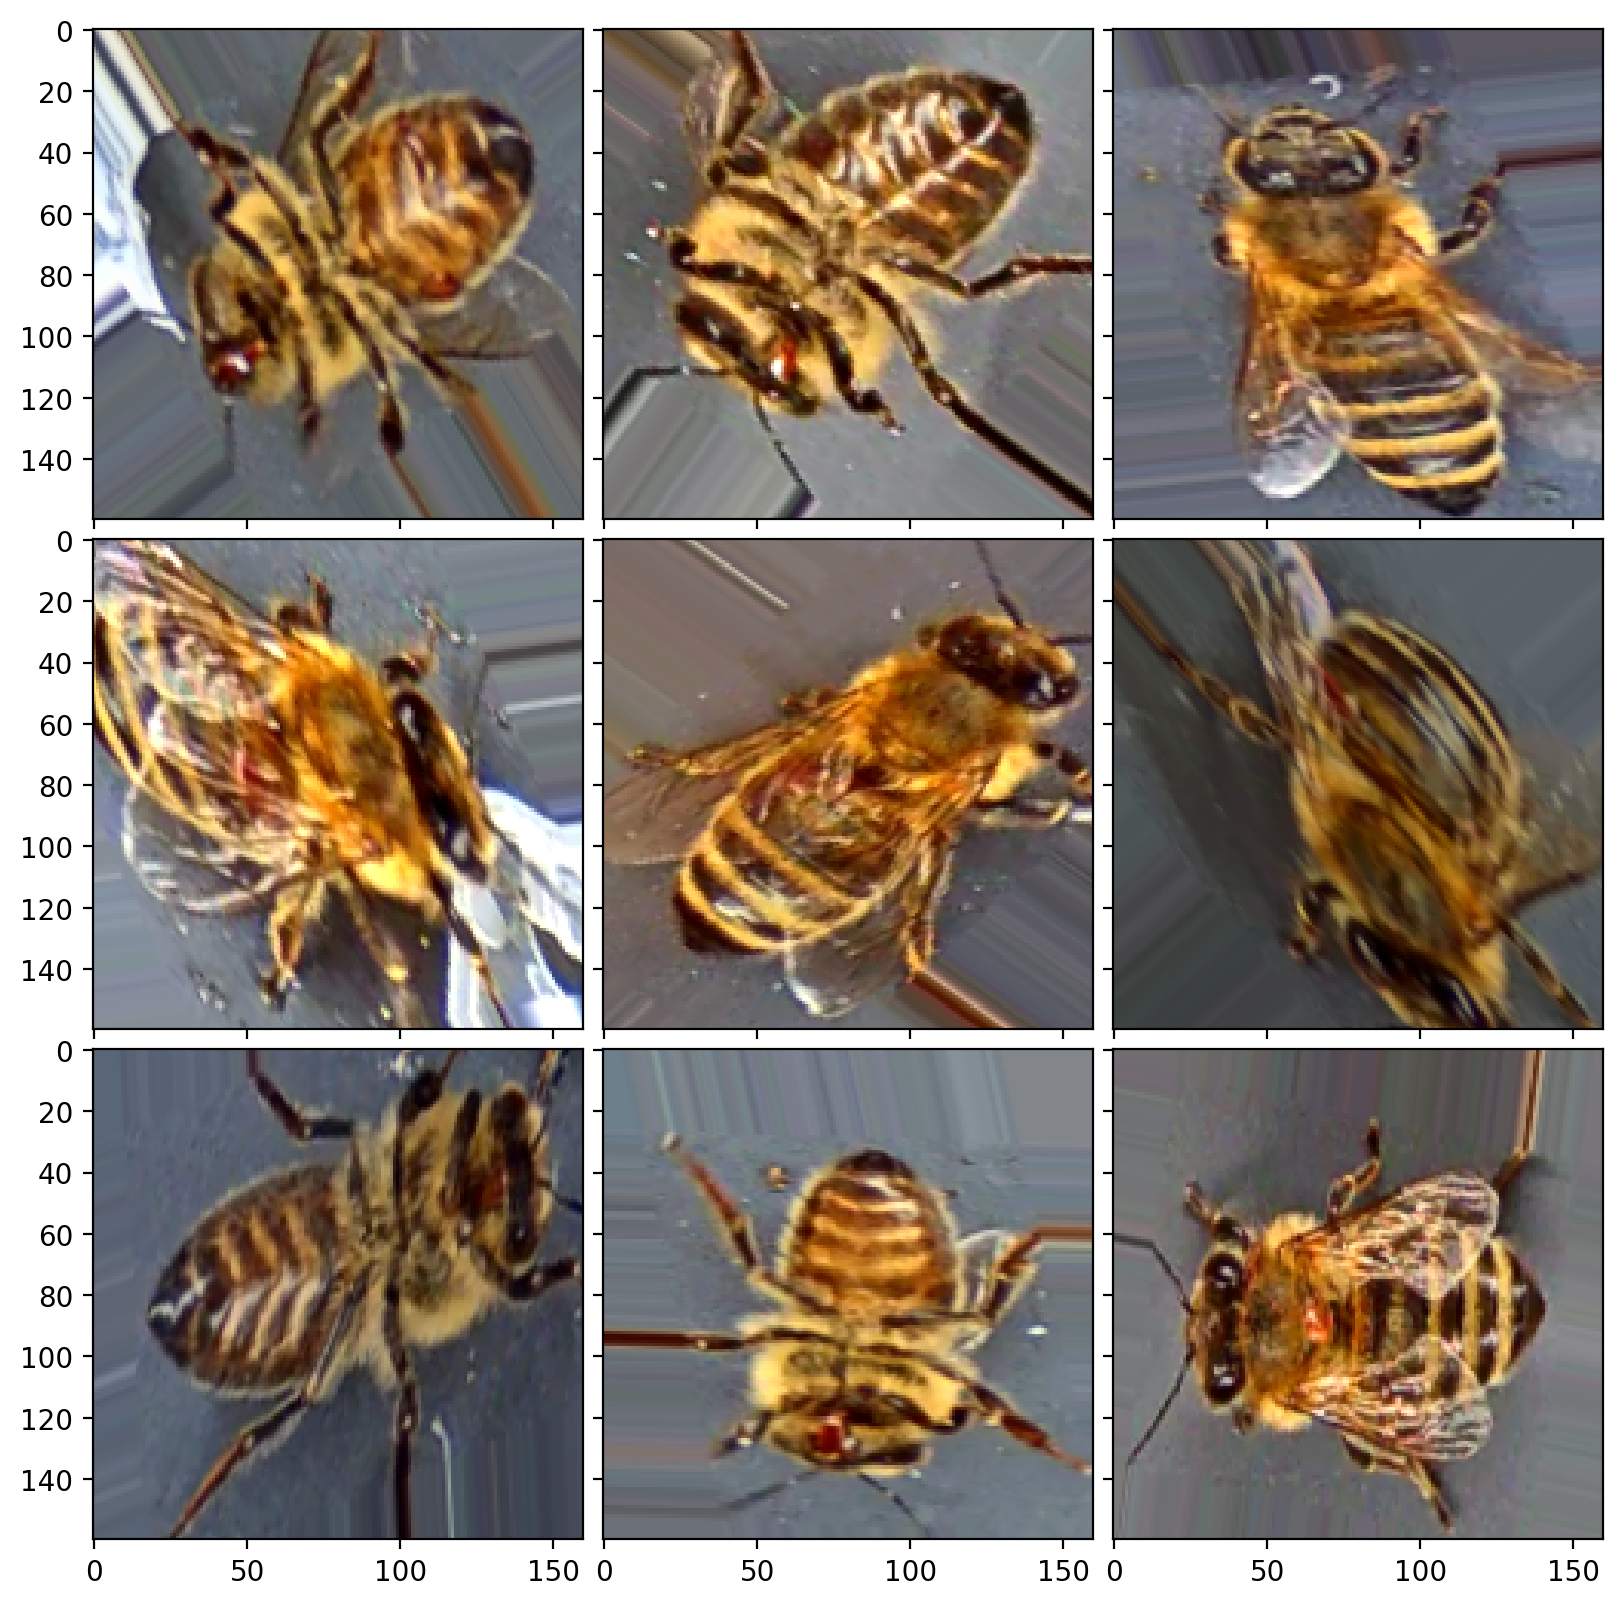
\includegraphics[width=13.5cm]{data_augmentation.png}
\caption{Augmented images}
\label{figure:data_augmentation}
\end{figure}

\section{Modeling}

As our starting point for transfer learning we chose the MobileNetV2 \cite{sandler2018mobilenetv2} architecture pretrained on ImageNet \cite{deng2009imagenet}. This architecture was chosen deliberately to ensure fast inference times on mobile devices and compatibilities with post-training quantization and \href{https://coral.ai/docs/edgetpu/models-intro/#supported-operations}{operations supported by the Coral Edge TPU}. To reduce the need for prior input preprocessing, a rescaling layer which multiplies the input by $\frac{1}{255}$ was added and the top of the network was replaced by a global average pooling layer followed by a single dense unit with a sigmoid activation function.

For each training phase the batch size was set to $32$, the optimizer was set to \textit{Adam} \cite{kingma2014adam} with $0.001$ as the inititial learning rate and the number of epochs was set to $50$ to ensure proximity to convergence. All models were checkpointed with highest validation accuracy. The training was performed with \href{https://github.com/tensorflow/tensorflow}{\textbf{tensorflow}} accessed via the \href{https://keras.io/api/}{\textbf{keras} API}.

\section{Optimizations}

Besides inference latency, inference time and power usage are the most important factors for edge deployment of machine learning models, with both being directly correlated to each other. Power efficiency constitutes a critical quality because embedded systems may be deployed in environments in which a continuous power source is not readily available, which may require the expensive endeavor of recharging the device by changing the battery by hand. To prepare for this scenario the models were optimized in two different ways.

\subsection{Quantization}

Quantization is a technique used to reduce inference time, reduce model size and achieve compatibility with certain hardware. Model operations, which are usually performed on floating point numbers, are converted to use lower precision data types such as 16-bit floats or 8-bit integers. Full integer quantization, where every parameter and operation is converted to use 8-bit integers, is needed for compatibility with many hardware accelerators and microcontrollers. 

To make use of the aforementioned advantages, all varroa mite detection models are additionally converted to their fully 8-bit quantized form after training and tested on the Raspberry.

\subsection{Edge TPU}

Tensor Processing Units are application specific chips which are designed to perform matrix multiplications at great speed and efficiency. For example, the \href{https://coral.ai/docs/edgetpu/faq/}{Coral Edge TPU} is an ASIC which is designed to provide fast and power efficient inferences on portable devices.

To provide the option of deploying the models with maximal inference efficiency, all quantized models were additionally compiled for the Coral Edge TPU and tested on the \href{https://coral.ai/products/dev-board/}{Coral Dev Board}.

\section{Results}

In this section we are going to inspect the results produced by our models in both a quantitative and qualitative way.

\subsection{Predictions}
To get an impression of how the classifiers perform on concrete instances real world data, samples of positively and negatively classified bee images were taken from the testing data. The samples are shown in figures \ref{figure:positive_predictions} and  \ref{figure:negative_predictions}. For both samples the predictions seem to be aligned with the physical reality.
 
\begin{figure}[H]
\centering
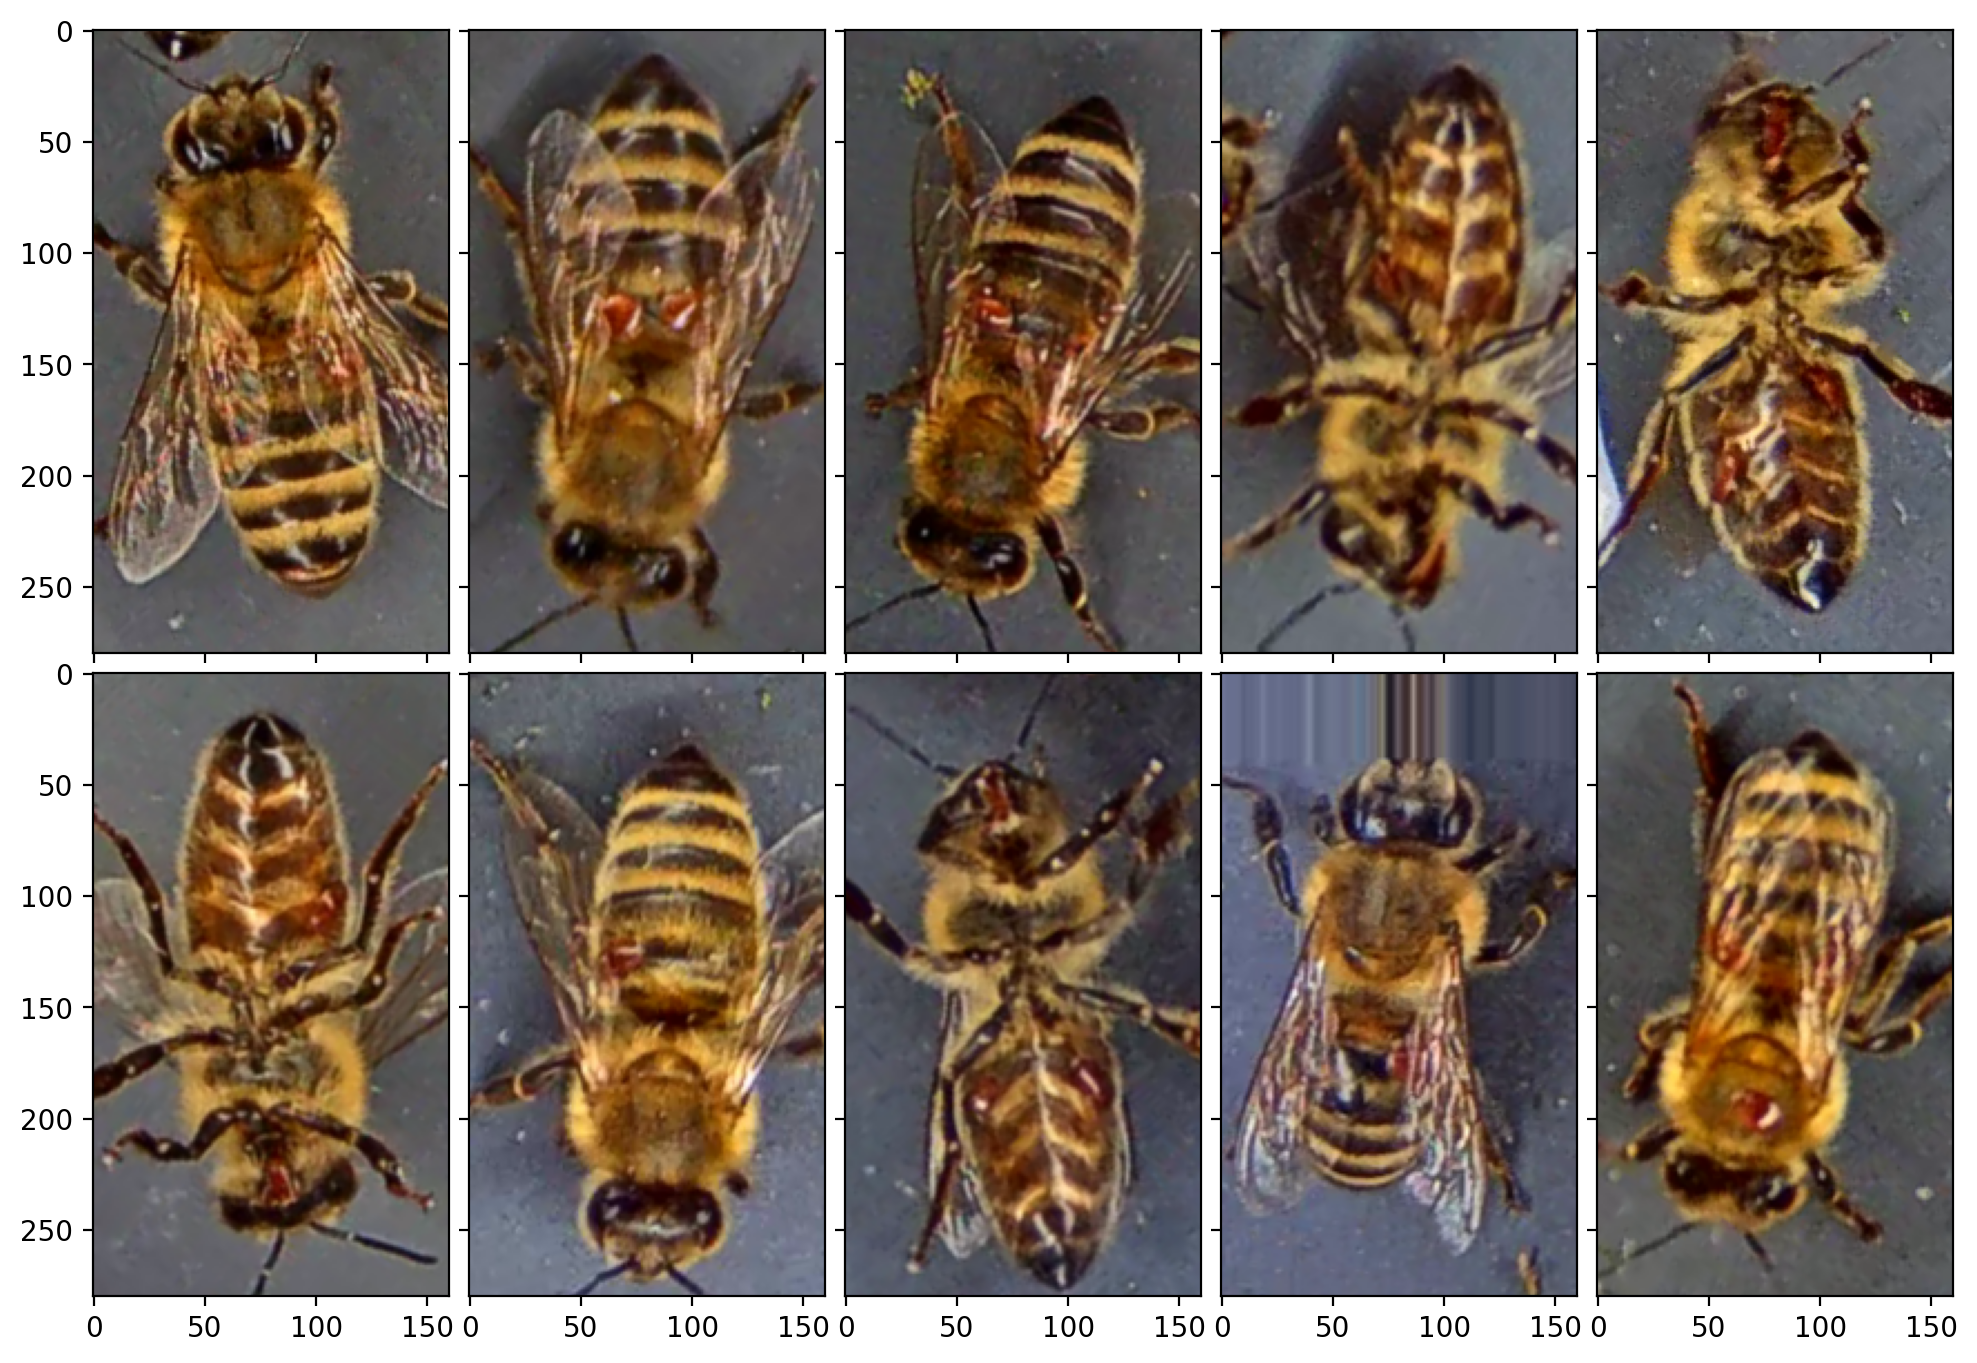
\includegraphics[width=13.5cm]{samples_positive.png}
\caption{Predicted positive}
\label{figure:positive_predictions}
\end{figure}

\begin{figure}[H]
\centering
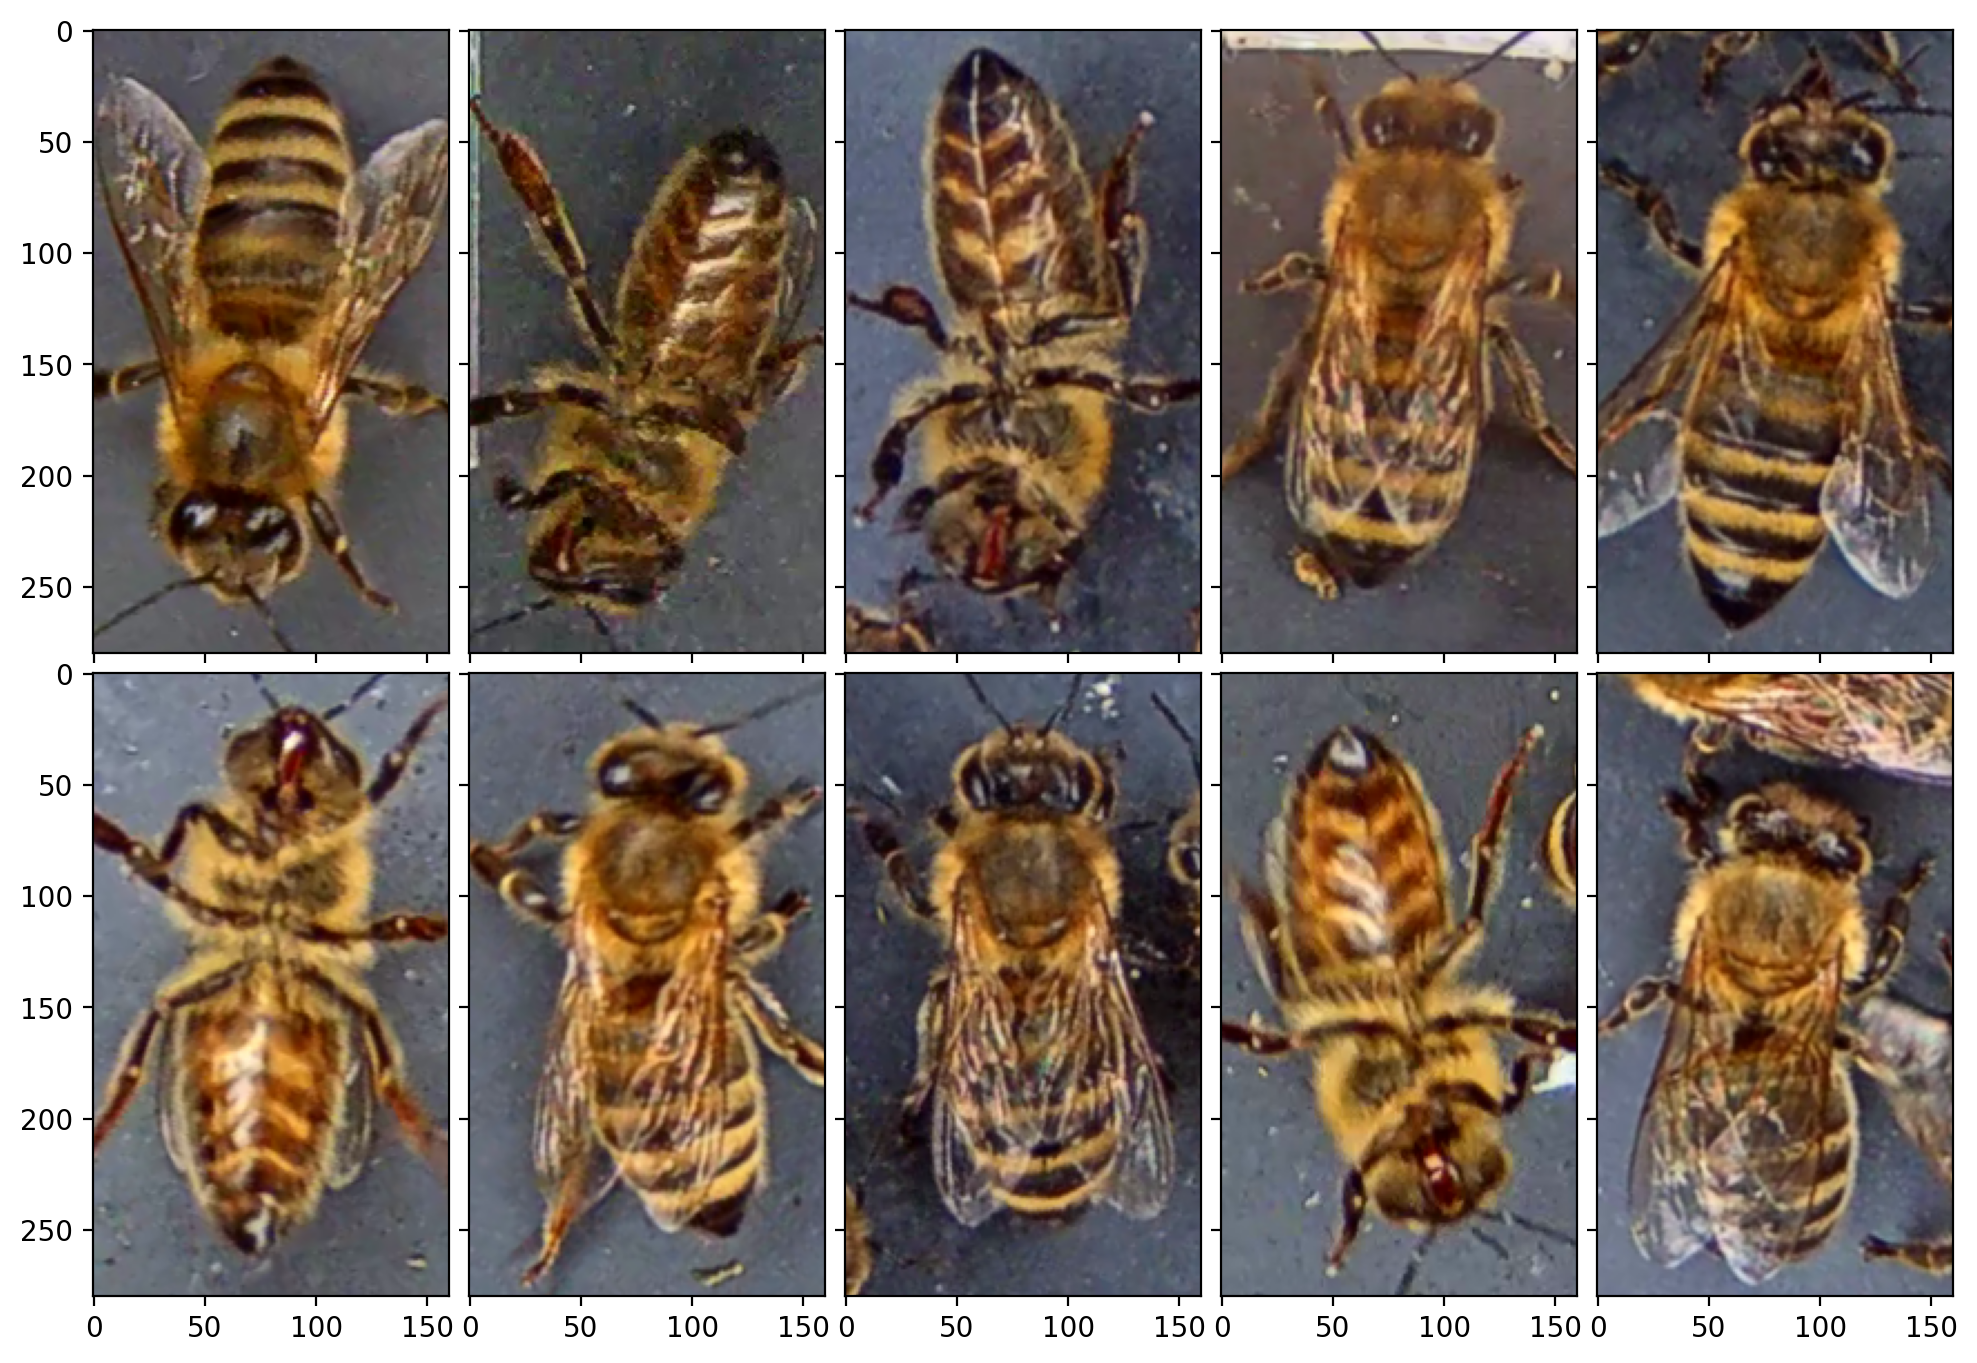
\includegraphics[width=13.5cm]{samples_negative.png}
\caption{Predicted negative}
\label{figure:negative_predictions}
\end{figure}

\subsection{Occlusion Sensitivities}

Even more confidence that the classifier picked up the right patterns can be gained by using an explainability technique called \textit{Occlusion Sensitivity}. This technique works by hiding patches of the image and observing how it affects the classification result for each location where the patch is hiding a part of the original image. For images which contain a single mite the prediction is impacted greatly if the patch occludes the mite, which can be seen by bright highlights. If an image contains multiple mites, then those highlights might not appear because the occlusion of a single mite does not affect the overall prediction.  Occlusion sensitivities generated with \href{https://github.com/sicara/tf-explain}{\textbf{tf-explain}} for a batch of $8$ images are displayed in figure \ref{figure:occlusion_sensitivity}. We can see that for the images in this sample our detector recognizes the individual mites as the most important feature.

\begin{figure}[H]
\centering
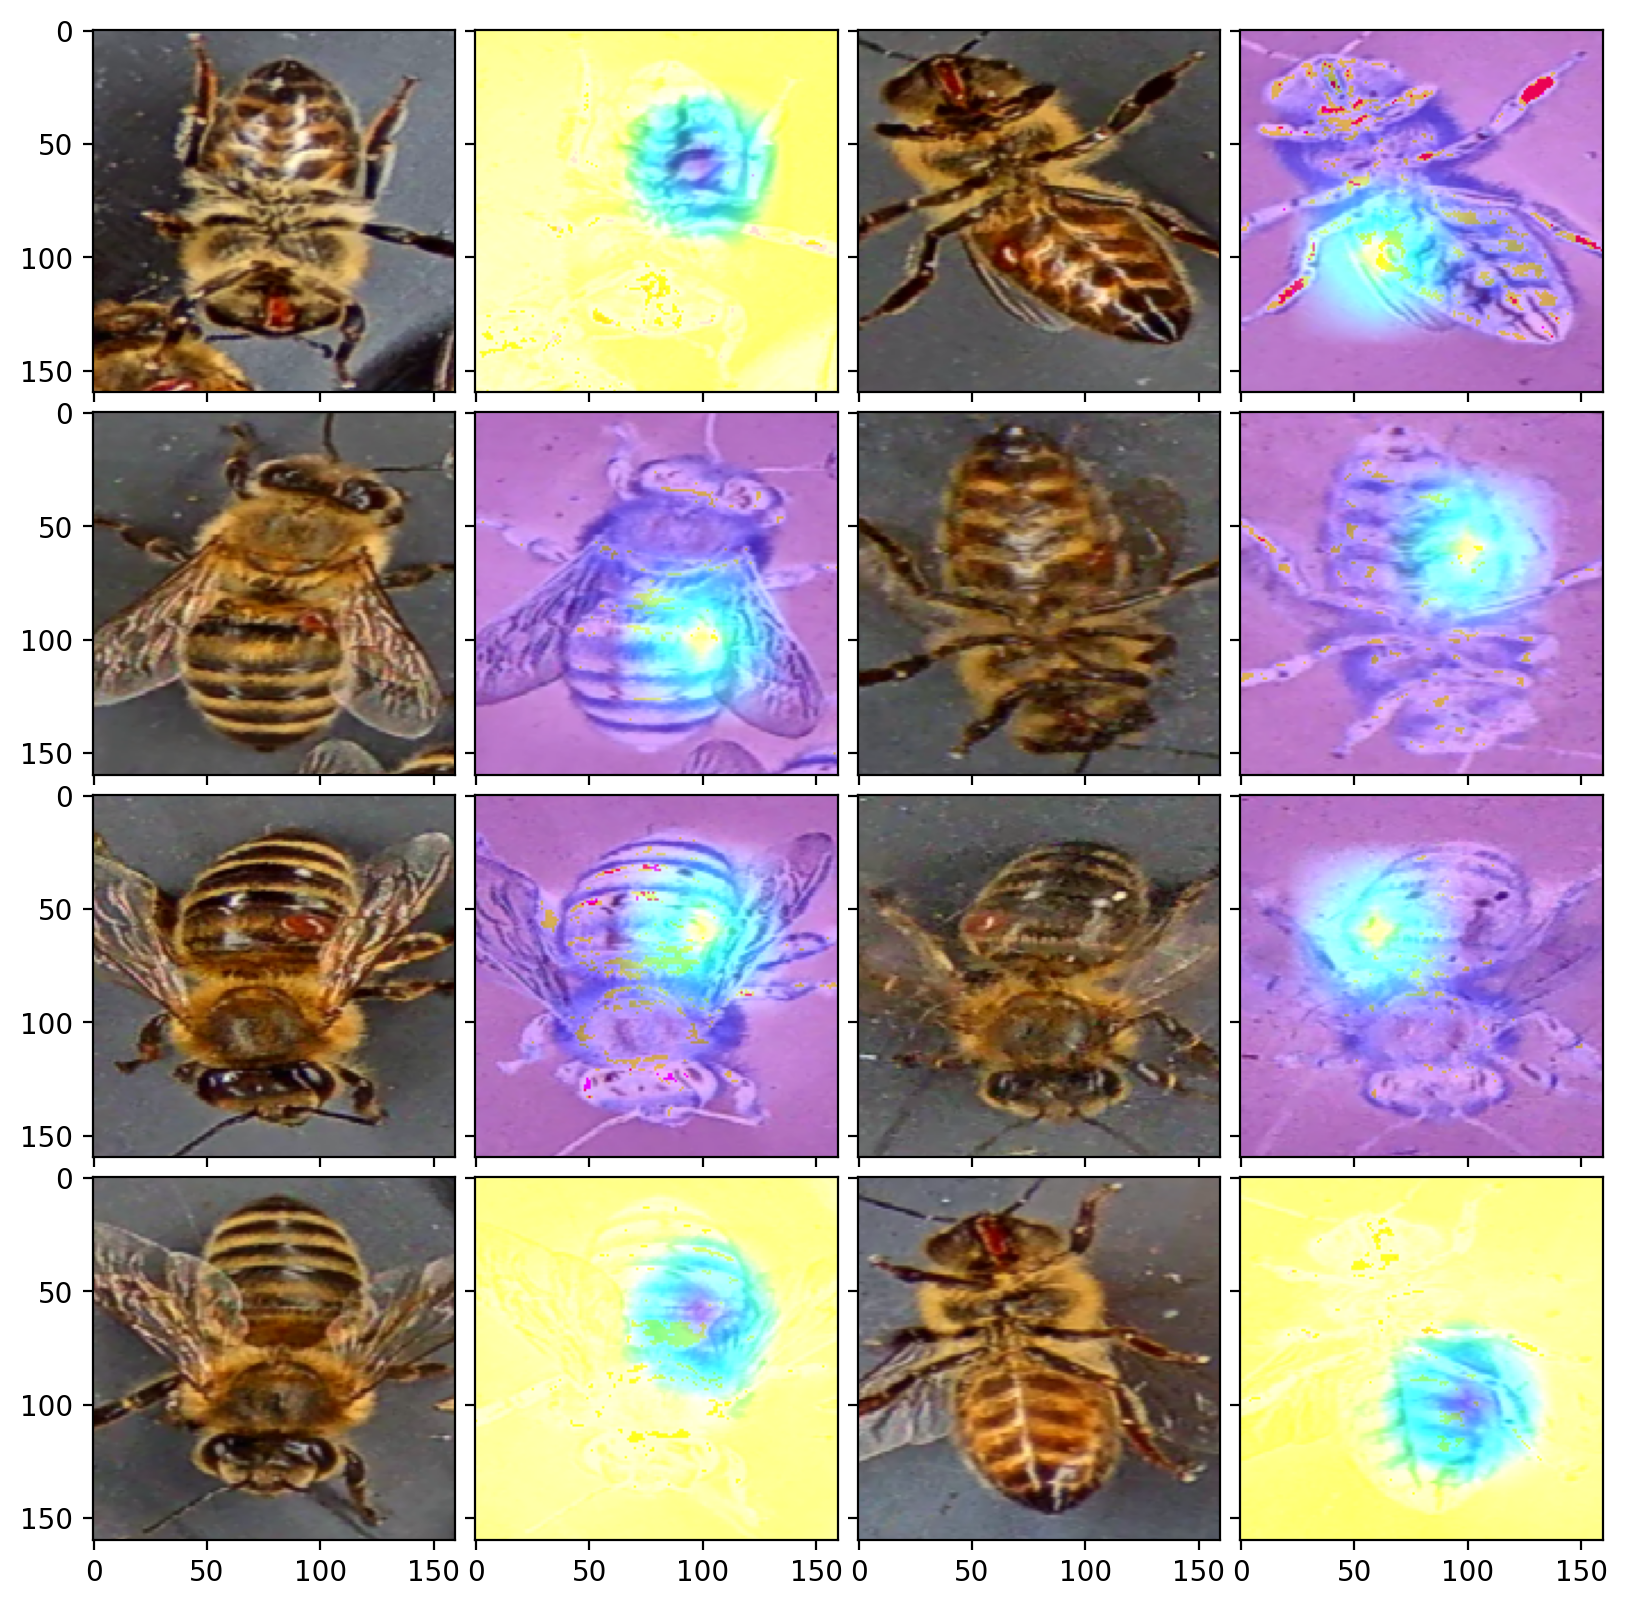
\includegraphics[width=13.5cm]{occlusion_sensitivity.png}
\caption{Occlusion sensitivities}
\label{figure:occlusion_sensitivity}
\end{figure}

\subsection{Classification Scores}

General prediction performance can be estimated by calculating classification metrics on the testing data. For the sake of completeness, all models were evaluated on the whole data set. The results are displayed in tables \ref{table:prediction_scores}, \ref{table:prediction_scores_quantized} and \ref{table:prediction_scores_edgetpu}. We can see that minor numerical disturbances are introduced by both post-training quantization and Edge TPU compilation. Overall, the prediction performance seems to be respectable. When comparing the scores of the $96 \times 96$ model to the other ones, a drop in performance is apparent. Even though the accuracies of both the $128 \times 128$ and $160 \times 160$ models are almost identical, the difference can be seen in the higher recall and lower precision score of the latter model, which means that the  $160 \times 160$  model is more aggressive with producing positive classifications. This could signify that it is a better model, because it classifies wrongly negatively labeled images as positive.

\begin{table}[H]
\centering
\begin{tabular}{@{}llllll@{}}
\toprule
Set  & Model & Accuracy & Precision & Recall & AUC \\ \midrule
train & 160\_160\_3\_mobilenetv2 & 0.9658 & 0.9629 & 0.9844 & 0.9845 \\
& 128\_128\_3\_mobilenetv2 & 0.9622 & 0.9734  & 0.9674 & 0.9738  \\
& 96\_96\_3\_mobilenetv2 & 0.9474 & 0.9540 & 0.9641 & 0.9724 \\ \midrule
validation & 160\_160\_3\_mobilenetv2 & 0.9552 & 0.9507 & 0.9808 & 0.9722  \\
& 128\_128\_3\_mobilenetv2 & 0.9552 & 0.9656 & 0.9643 & 0.9633 \\
& 96\_96\_3\_mobilenetv2  & 0.9490 & 0.9552 & 0.9657 & 0.9625 \\ \midrule
test & 160\_160\_3\_mobilenetv2 & 0.9441 & 0.9394  & 0.9754 & 0.9695 \\
& 128\_128\_3\_mobilenetv2 & 0.9441 & 0.9550 & 0.9576 & 0.9570 \\
& 96\_96\_3\_mobilenetv2 & 0.9249 & 0.9352 & 0.9480 & 0.9533 \\ \bottomrule
\end{tabular}
\caption{Prediction scores}
\label{table:prediction_scores}
\end{table}

\begin{table}[H]
\centering
\begin{tabular}{@{}llllll@{}}
\toprule
Set & Model & Accuracy & Precision & Recall & AUC \\ \midrule
train & 160\_160\_3\_mobilenetv2   & 0.9647   & 0.9599    & 0.9859 & 0.9833 \\
& 128\_128\_3\_mobilenetv2   & 0.9620   & 0.9731    & 0.9674 & 0.9715 \\
& 96\_96\_3\_mobilenetv2     & 0.9492   & 0.9579    & 0.9630 & 0.9731 \\ \midrule
validation & 160\_160\_3\_mobilenetv2   & 0.9561   & 0.9520    & 0.9808 & 0.9718 \\
& 128\_128\_3\_mobilenetv2   & 0.9561   & 0.9631    & 0.9684 & 0.9598 \\
& 96\_96\_3\_mobilenetv2     & 0.9517   & 0.9578    & 0.9670 & 0.9628 \\ \midrule
test & 160\_160\_3\_mobilenetv2   & 0.9424   & 0.9358    & 0.9767 & 0.9701 \\
& 128\_128\_3\_mobilenetv2   & 0.9432   & 0.9524    & 0.9590 & 0.9591 \\
& 96\_96\_3\_mobilenetv2     & 0.9293   & 0.9392    & 0.9508 & 0.9536 \\ \bottomrule
\end{tabular}
\caption{Prediction scores for quantized models}
\label{table:prediction_scores_quantized}
\end{table}

\begin{table}[H]
\centering
\begin{tabular}{@{}llllll@{}}
\toprule
Set & Model & Accuracy & Precision & Recall & AUC \\ \midrule
train & 160\_160\_3\_mobilenetv2 & 0.9658   & 0.9618    & 0.9856 & 0.9841 \\
& 128\_128\_3\_mobilenetv2 & 0.9624   & 0.9737    & 0.9674 & 0.9712 \\
& 96\_96\_3\_mobilenetv2   & 0.9489   & 0.9581    & 0.9621 & 0.9726 \\ \midrule
validation & 160\_160\_3\_mobilenetv2 & 0.9561   & 0.9532    & 0.9794 & 0.9718 \\
& 128\_128\_3\_mobilenetv2 & 0.9534   & 0.9604    & 0.9670 & 0.9592  \\
& 96\_96\_3\_mobilenetv2   & 0.9525   & 0.9591    & 0.9670 & 0.9628 \\ \midrule
test & 160\_160\_3\_mobilenetv2 & 0.9450   & 0.9406    & 0.9754 & 0.9714 \\
& 128\_128\_3\_mobilenetv2 & 0.9467   & 0.9552    & 0.9617 & 0.9579 \\
& 96\_96\_3\_mobilenetv2   & 0.9284   & 0.9391    & 0.9494 & 0.9547 \\ \bottomrule
\end{tabular}
\caption{Prediction scores for quantized models compiled for Edge TPU}
\label{table:prediction_scores_edgetpu}
\end{table}

\subsection{Decision Curves}
Receiver operating characteristic curves are often used to demonstrate the trade-offs between the true positive rate and the true negative rate at various decision thresholds. Similarly, precision-recall curves demonstrate the trade-offs between precision and recall.  The curves constructed for our models are displayed in figures \ref{figure:roc_curves} and \ref{figure:precision_recall_curves}. A larger area under the curve (AUC) signifies a better trade-off between the respective metrics and with that a better overall classification performance.

\begin{figure}[H]
\centering
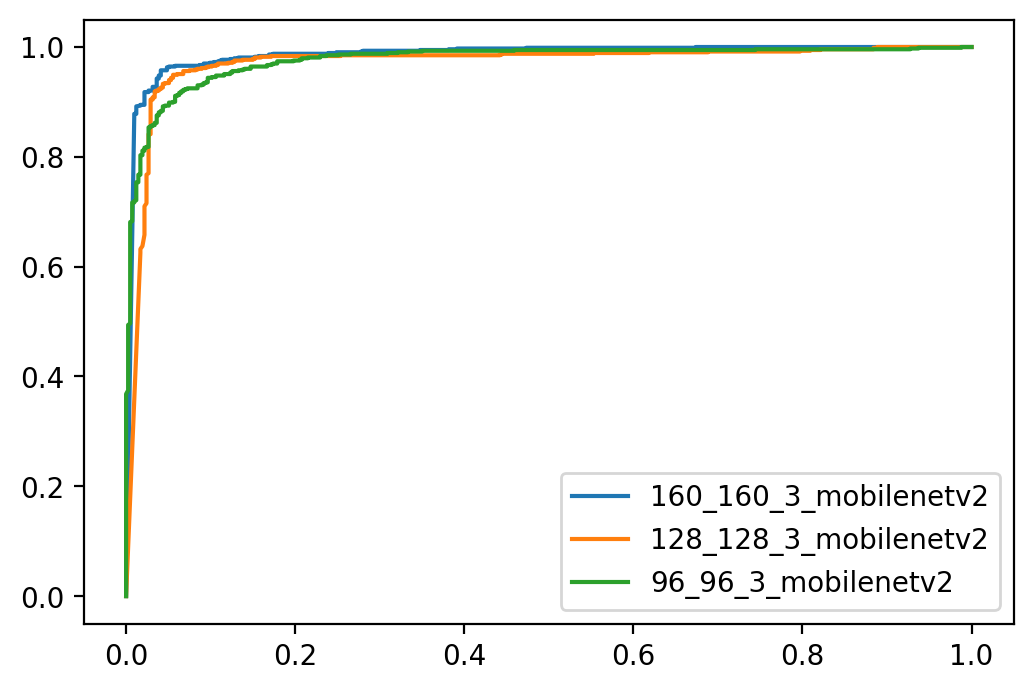
\includegraphics[width=13cm]{roc_curves.png}
\caption{ROC curves}
\label{figure:roc_curves}
\end{figure}

\begin{figure}[H]
\centering
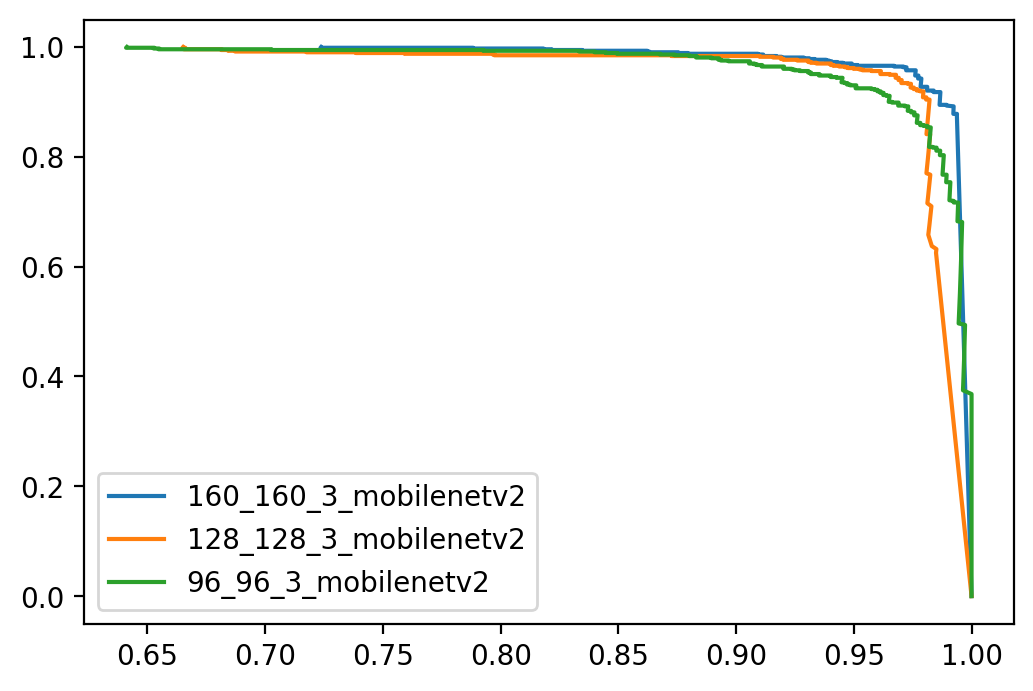
\includegraphics[width=13cm]{precision_recall_curves.png}
\caption{Precision-recall curves}
\label{figure:precision_recall_curves}
\end{figure}


\subsection{Inference Times}

To estimate performance in deployment scenarios, mean inference times were measured for the \href{https://www.raspberrypi.org/products/raspberry-pi-4-model-b/specifications/}{Raspberry Pi 4} and  the \href{https://coral.ai/products/dev-board/#tech-specs}{Coral Dev Board}. The results are displayed in tables \ref{table:inference_times}, \ref{table:inference_rates} and \ref{table:inference_times_per_input_size}. The inference rates for Coral Dev Board are without a doubt high enough to be practically viable. On the Raspberry Pi 4 the inference rates are more modest but could still be enough if the camera producing the input is set up in a way which maximizes the time-span over which a particular bee is visible. On the Raspberry Pi 4 the inference times scale almost linearly with the input size, while on the Coral Dev Board the step from an input resolution of $128 \times 128$ to $96 \times 96$ has almost no effect on inference speed.

\begin{table}[H]
\centering
\begin{tabular}{@{}lll@{}}
\toprule
                         & Coral Dev Board    & Raspberry Pi 4     \\ \midrule
160\_160\_3\_mobilenetv2 & 1.974 & 72.524  \\
128\_128\_3\_mobilenetv2 & 1.258 & 47.954  \\
96\_96\_3\_mobilenetv2   & 1.158  & 30.601 \\ \bottomrule
\end{tabular}
\caption{Inference times in milliseconds}
\label{table:inference_times}
\end{table}

\begin{table}[H]
\centering
\begin{tabular}{@{}lll@{}}
\toprule
                         & Coral Dev Board   & Raspberry Pi 4     \\  \midrule
160\_160\_3\_mobilenetv2 & 506.58  & 13.79 \\
128\_128\_3\_mobilenetv2 & 794.60 & 20.85  \\
96\_96\_3\_mobilenetv2   & 863.70 & 32.68 \\ \bottomrule
\end{tabular}
\caption{Inferences per second}
\label{table:inference_rates}
\end{table}

\begin{table}[H]
\centering
\begin{tabular}{@{}lll@{}}
\toprule
                         & Coral Dev Board        & Raspberry Pi 4        \\ \midrule
160\_160\_3\_mobilenetv2 & 2.57e-05 & 9.44e-04 \\
128\_128\_3\_mobilenetv2 & 2.56e-05  & 9.76e-04 \\
96\_96\_3\_mobilenetv2   & 4.19e-05   & 1.11e-03  \\ \bottomrule
\end{tabular}
\caption{Inferences times per input size}
\label{table:inference_times_per_input_size}
\end{table}

\section{Conclusion}
Based on the results we can conclude that the approach is practically viable in respect to detection accuracy and run time efficiency. We think that a solid ground truth based on maximal label certainty, particularly regarding data labeled as negative, would combat the cognitive dissonance induced to the network, ultimately leading to a more clear cut decision boundary. We are convinced that this would significantly increase detection accuracy on hard images to a point at which classifier performance would surpass predictions made by humans by a significant margin.

In deployment, an approach to make detection more robust against misleading signals (such as the position of a leg looking like a mite on the side of the thorax) could be to conservatively estimate how many frames a particular bee should be visible to the camera depending on the camera setup and maximal movement speeds and average the prediction results for those frames.

\bibliographystyle{unsrt}
\bibliography{references}

\end{document}
